\chapter{Implementation}
\label{chap:implementation}
\todo{lots of figures and screenshots should be used here}
\todo{Grammarly me}
This chapter consists of implementation details for all relevant redirected walking components as well as an overview of the game design for the developed ''Ensemble Retriever'' game. The game design overview is used to provide examples and documentation on how distractors have been fully integrated into the experience itself. 

\section{Open Source Repository - GitHub}
The source code and project assets for Ensemble Retriever can be found in a publicly available GitHub Repository~\cite{projectRepository}. It should be noted that the game itself is an extension of a small prototype that was previously developed for the IMT4894 - Advanced Project Work course. This prototype consisted of no redirected walking elements and simply featured a battle in VR against an angry contrabass enemy. The majority of the source code has needed to be rewritten or refactored to facilitate a more generic architecture that supports the larger scope of the current game.  
\todo{briefly mention what the prototype actually contained}
\subsection{Licensing and Attribution}
\todo{not sure whether it should be in this chapter or general methods}

Ensemble Retriever makes liberal use of royalty free assets as a means to fasten then development time of the game. As such, it is also necessary to properly provide attribution to these assets. In general, each royalty free asset in the repository includes a corresponding license file which details the specific license that applies to it. The following list gives an overview of the royalty free assets that were used for the project:
\begin{itemize}
    \item Most Particle effects
    \item Fonts
    \item Some 3D Models like hats/crowns, conducting baton, objective arrow and the cave walls in the ''Hall of The Mountain King''.
    \item Skybox
    \item Music
    \item Sound effects
\end{itemize}
Anyone who is interested in reusing or extending the project need to follow the licensing terms that apply for all of these assets. There are also specific 3D models that were reused from a previous project with permission from their creator, Yjie Zhou. These can be found in the \emph{''Assets/Meshes/BlenderAssets/''} folder of the repository and include:
\begin{itemize}
    \item All instrument 3D models
    \item The virtual environment
\end{itemize}\todo{Reusing the project as is is most likely fine, but further extension for these elements might not be allowed}
Extension or reuse of these assets are not permitted in other work and need to be replaced as the permission was given to reuse these assets for this project specifically. All other assets were developed specifically for the Ensemble Retriever game and include:
\begin{itemize}
    \item All game logic + extensions to the Redirected Walking Toolkit
    \item All animations
    \item All sprites/textures with the exception of an image of a HTC Vive Controller
    \item All voice acting
    \item Some particle effects like player attacks, projectile blocks and sweating particles for The Mountain King 
\end{itemize}
These elements of the game are under a MIT License and allows for reuse/extension as long as the license terms are held. 

\section{Redirected Walking Toolkit - Extended Code Architecture}
As part of developing Ensemble Retriever, Azmandian et al's Redirected Walking Toolkit~\cite{azmandian2016redirected} has been extended to support the usage of distractors and any other interfacing that the game has required. A chart showing the general additions to the toolkit's architecture can be found in Figure~\todo{ADD/MAKE ME}. The general thought process throughout the development of these extensions was to not do any major changes to the toolkit itself for the sake of keeping its modular structure. If functionality could be build on top of parts of the toolkit, then inheritance was used. If any part of the toolkit required major changes, it would be copied to a separate file which these modifications were written in. As far as minor changes are concerned, these mostly consisted of changing some data access properties of variables to allow for easier communication between classes.

As seen in Figure~\todo{ADD/MAKE}, the toolkit has been extended with the following components:
\begin{itemize}
    \item RedirectionManagerER which extends RedirectionManager to facilitate communication and management between new components
    \item The ''Align Centre To Future''(AC2F) Redirector
    \item The ''Pause - Turn - Centre'' Resetter
    \item The Distractor Trigger System
    \item ExperimentManager which handles data collection and experiment management
    \item GainIncrementer which is used as part of experiment 1
\end{itemize}

Each of these will be further detailed in the following sections. 

\section{Managing The Extended Architecture}
* RedirectionManagerER details in general
* Overall structure and communication between components.
* Switching between S2C and AC2F
* Position sampling

* Double check these
* 0.5m away from wall = reset
* 1.5m away from wall = distractor
* 1m buffer between distractor trigger and reset


\section{The ''Align Centre to Future'' Redirector}
\begin{figure}[htbp]
  \centering
  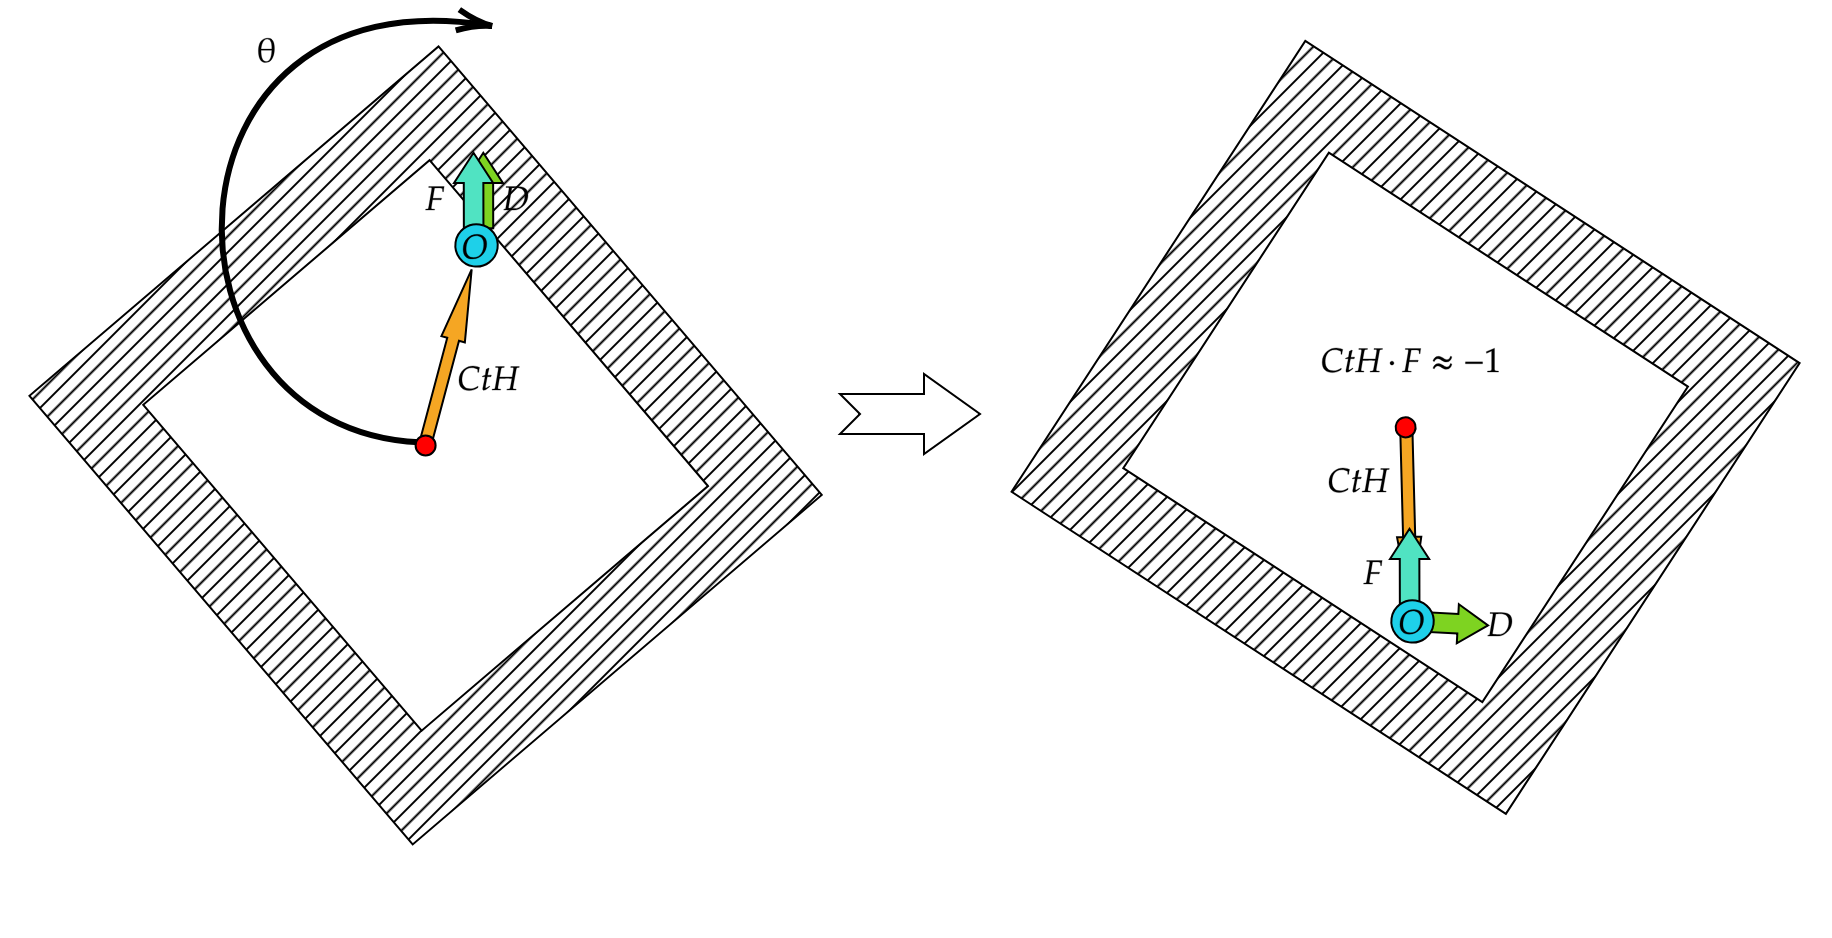
\includegraphics[width=\textwidth]{figures/graphs/AC2F.png}
  \caption[Align Centre to Future Algorithm Example]{AC2F aims to choose the rotation gains that brings the physical centre to head ($CtH$) vector in alignment with the future virtual walking direction ($F$) of the user. The user's current facing direction ($D$) is not used other than setting the value of $F$ as the algorithm starts. The origin of this reorientation is at the position of the user ($O$)}
  \label{fig:ac2f}
\end{figure}

* The way that the real world ''rotates'' depends on what gain is applied to the user and what direction they are moving their head in. 
   * The optimal gain is directly calculated at runtime, but it is technically possible to just choose one depending on the direction you want to rotate relative to what direction the user's head moves in


* Figure~\ref{fig:ac2f}
* Code specific implementation details. 
* Based on what Peck et al. + Chen and Fuchs have mentioned in their work. 
   * No source code was available from their work, as such AC2F is somewhat based on Azmandian et al.'s S2C implementation, but the final result is fairly different from S2C.
   
   
* Smoothing, moving between positive and negative gains
   * Dealing with edge cases, stopping motions
   * A threshold is needed to decide whenever a rotation is large enough to apply gains or not.
      * Since the head naturally vibrates slightly as well as tracking not being completely perfect, we do not want to let participants experience rotation gains as their head is still.
      * This threshold method does cause some issues if we completely disable gains at the end of a head rotation as it creates a jarring difference between applied gains and 0 gains.
      * As such, it would be ideal to also smooth out the stopping motion of head rotations.


\section{The ''Pause - Turn - Centre'' Resetter}\label{sec:pauseturncentre}
* Inspired by freeze turn (CITE creator)
* Also takes inspiration from what Sra et al. have mentioned
   * Limiting visibility makes changes less noticable
   * In this case, the virtual world is "paused", resulting in a rotation gain of 0, but this is masked by mostly fading it to black and overlaying a representation of the physical space on top. 
* Clipping problem
   * How is it solved?
       * Double camera solution, forcing different depth levels so one camera always will draw over what the other does
   * What are the pros/cons of this solution?
      * Easy to implement
      * Costs some performance
         * Especially if post processing is used. 4 cameras in total, each needing to do post processing is costly.
            * There is some granularity here though. For example it is possible to control what PP is applied to the virtual/physical spaces. Less can be applied to the physical space as it is not seen as often.

\subsection{Pausing the Game Using ''Pause - Turn - Centre''}
* All dynamic objects in the game use a specific pausable class as their parent. 
   * This includes any projectiles, distractors and other animated components.
* The redirectionManager is then able to find a list of all objects that derive from this pausable class when resetting is necessary. It then triggers a callback for each of these so they can take care of pausing their own behaviour. 

\section{Supporting the Y axis in the RDW toolkit}
   * Basically a bugfix to the way the toolkit worked
   * an issue with the body follower not working with the Y axis. 
   * This change was put into the toolkit itself as it was more of a bug rather than a major change.

\section{Game Design Overview of Ensemble Retriever} 
\begin{figure}[tbph]
    \centering
    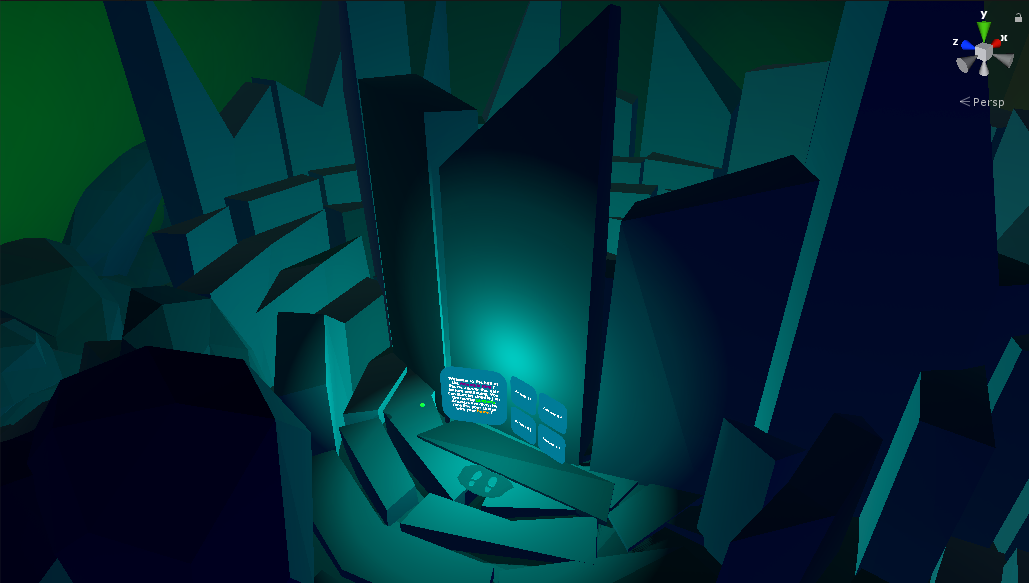
\includegraphics[width=0.5\textwidth]{figures/screenshots/HallOfTheMountainKingKindaLowRes.png}
    \caption[Screenshot of the ''Hall of The Mountain King'']{This screenshot from the Unity scene view shows the ''Hall of The Mountain King'' with the quiz section that the player has to answer.}
    \label{fig:mkhallWithWall}
\end{figure}

\begin{figure}[tbph]
    \centering
    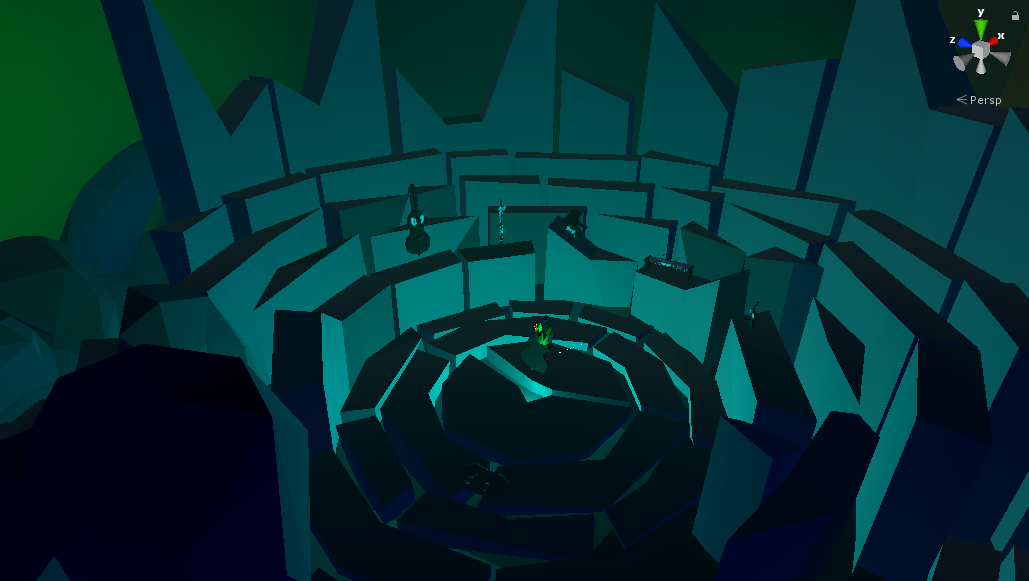
\includegraphics[width=0.5\textwidth]{figures/screenshots/HallOfTheMountainKing2KindaLowRes.png}
    \caption[Screenshot of the ''Hall of The Mountain King'' Without the Quiz Wall]{This screenshot from the Unity scene view shows the ''Hall of The Mountain King'' after the player has answered the quiz section in the game. This is where the Mountain King is fought.}
    \label{fig:mkhallWithoutWall}
\end{figure}
In Ensemble Retriever, the player takes the role of a conductor whose goal is to retrieve the ''Mountain King'', which is an instrument that has disappeared from their ensemble. In order to find the ''Mountain King'', the player has to walk around in a large virtual environment and ask the local residents for clues before they can enter the ''Hall of The Mountain King'' seen in Figure~\ref{fig:mkhallWithWall} and \ref{fig:mkhallWithoutWall}. Throughout the player's exploration of the virtual world, they are attacked by various distractor enemies which have to be defeated to gain experience points and progress the game. These battles consist of having the player use their contrabass shield to absorb enemy projectiles. Once enough projectiles have been absorbed, the player is able to counterattack with their magical conductor baton. The game culminates with a battle against the ''Mountain King'' that tests the player's skill and abilities which they have trained throughout their battles with distractor enemies.  

The following sections provides a more detailed context on the game itself and how distractors have been fully integrated into the experience.

\subsection{Virtual Environment}
* \todo{More Pictures! This one might change right before ex 1 if it takes too long to walk so no need write this until after that}
* Can show roughly how many metres the user has to walk to reach the portal etc. Top down views of the world relative to physical space and so on. 

\subsection{Game Flow}
\todo{Can probably add some pictures}
This section provides an outline of the flow of Ensemble Retriever and how the game progresses throughout a play session. 

Ensemble Retriever starts off with a tutorial that teaches the player the basics of the game. It provides information on the context/story, the player's goal, how to deal with reorientation resets, how to fight enemies and what to do if they are lost. In experiment 1, the tutorial also provides information on what the player should do if they notice they are being redirected. 

After the tutorial is finished, the game transitions to a walking phase where the player tries to reach the ''Hall of The Mountain King'' while being encouraged to visit three green fireflies that provide hints which will be relevant for a later part of the game. As the player walks around in this phase, distractor enemies will appear once they hit the maximum safe distance away from the centre. These enemies need to be defeated to progress and award experience points that the player can use to either upgrade the size of their contrabass shield or the damage that their conducting baton does. It should be noted that the fireflies fade away during battles to prevent their salience from potentially affecting the attention of the player since this could result in lower concentration~\cite{sitzmann2018saliency}. The walking phase of Ensemble Retriever is finished once the player enters the portal to the ''Hall of The Mountain King''. 

Once the player enters the ''Hall of The Mountain King'', any redirection gains are disabled. This is to allow the player to spend the last few minutes of the game getting used to normal head rotations before taking off the HMD. Inside the hall, the player has to answer a multiple choice quiz which asks questions based on the previous hints that could have been acquired from fireflies in the walking phase. The quiz itself cannot be failed, but the final score that the player is given ties with how many correct answers they give. The quiz itself has three questions in total.

Once the quiz is finished, the player will have to fight against the ''Mountain King''. This is a longer battle where the ''Mountain King'' will use combinations of all previous attacks that distractor enemies have been using to challenge the player. Once the ''Mountain King'' has been defeated, the game is finished and the player will be shown their scores which consists of four components:
\begin{enumerate}
    \item Time Score (How long it took to finish the game. Shorter times means higher scores)
    \item Damage Score (How much damage the player has taken in total. Less damage means higher scores)
    \item Quiz Score (How many correct quiz answers the player has gotten)
    \item Total Score
\end{enumerate}

\section{Fully Integrating Distractors with Game Mechanics}
\begin{figure}[tbph]
    \centering
    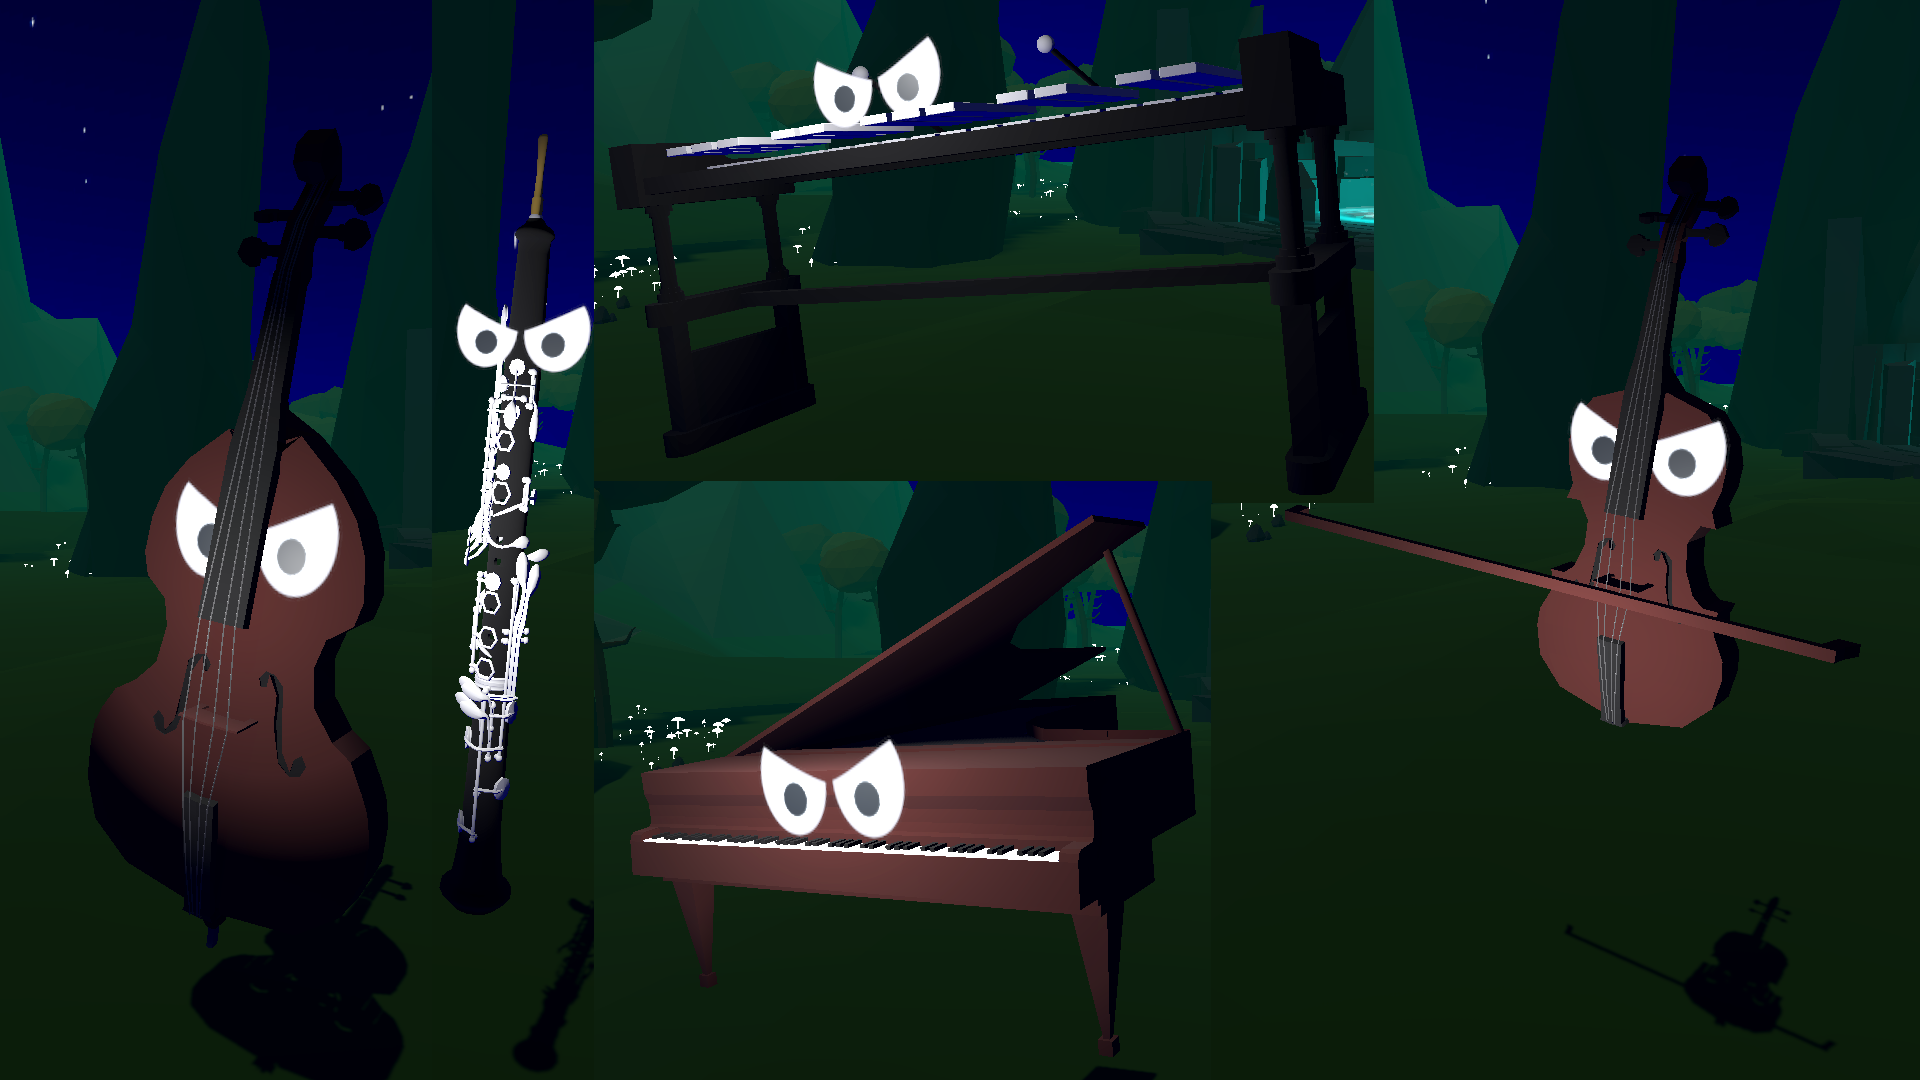
\includegraphics[width=1\textwidth]{figures/screenshots/Distractors.png}
    \caption[The Distractors of Ensemble Retriever]{These are the five distractor enemies that are employed in the Ensemble Retriever game.}
    \label{fig:allDistractors}
\end{figure}

The development resource budget of Ensemble Retriever was fairly small(\textasciitilde1.25 months). As such, in order to have a reasonable scope and allowing for as much code/asset reuse as possible, the main mechanic that was decided to fully integrate with distractors was the enemy encounters in the game. Since the AC2F algorithm relies on rotation gains, the goal of using distractors in this case was to make the player move their head around as much as possible. Ensemble Retriever currently consists of five enemy distractors which can be seen in Figure~\ref{fig:allDistractors}. If we look back to the taxonomy of distractors which was presented in Section~\ref{sec:distractorTaxonomy}, these can be considered as explicit, concrete distractors that are fully integrated into the experience. In this case, the distractors are considered explicit as the player is told they have to fight them. 

From a game design point of view, their use can be seen as ''random'' enemy encounters which is a common mechanic in role playing games. Instead of actually being random though, these enemy encounters trigger once the player has reached the maximum safe distance away from the centre of their physical tracking space. 

Once an enemy encounter starts, one of the five possible distractors are randomly chosen from a list. The chosen distractor is then removed from this list so it cannot be chosen again for some time. Once all distractor enemies have been chosen from the list, it is then repopulated with all five again. In the worst case scenario, this means that the same distractor might show up as the next enemy right after the list has been repopulated. The rationale for this approach is to avoid situations where the same distractor can show up too many times in a short space of time, potentially annoying the player due to limited variety as mentioned by Sra et al.~\cite{sra2018vmotion}. 

Each of the five distractor enemies rely on projectile attacks that have three potential movement speeds as well as a unique property per type of distractor. Before attacking, the distractor will make use of two telegraphs: one for the type of projectile it will attack with and one for how fast it will be. These telegraphs make use of both animation and audio cues, allowing the player to learn and identify the different types of attacks that are used so they can prepare accordingly. 

A standard enemy encounter consists of two phases: a tutorial phase and a proper battle phase. During the tutorial phase, the distractor will use its different attacks in order to teach the player its capabilities. In this phase, the distractor will not move away from its initial position. Once the player manages to counterattack the distractor, the real battle begins. During the battle phase, the distractor will randomly choose an angle between -360 and 360 degrees from the player after each attack, and rotate around them. The attack order will at this point also either be random or predetermined depending on the type of distractor. This forces a fair amount of head rotation from the player as they need to keep track of where the distractor moves and where their projectile attacks are. This also makes good use of the full 360 degree space that virtual reality allows while providing many opportunities for applying rotation gains.    

The following sections will describe and detail each distractor that exists in Ensemble Retriever. It should be noted that the screenshots of these were taken from the debug mode of the game, hence why the conductor baton and shield are in fixed screen positions.

\subsection{The Contrabass}
\begin{figure}[tbph]
    \centering
    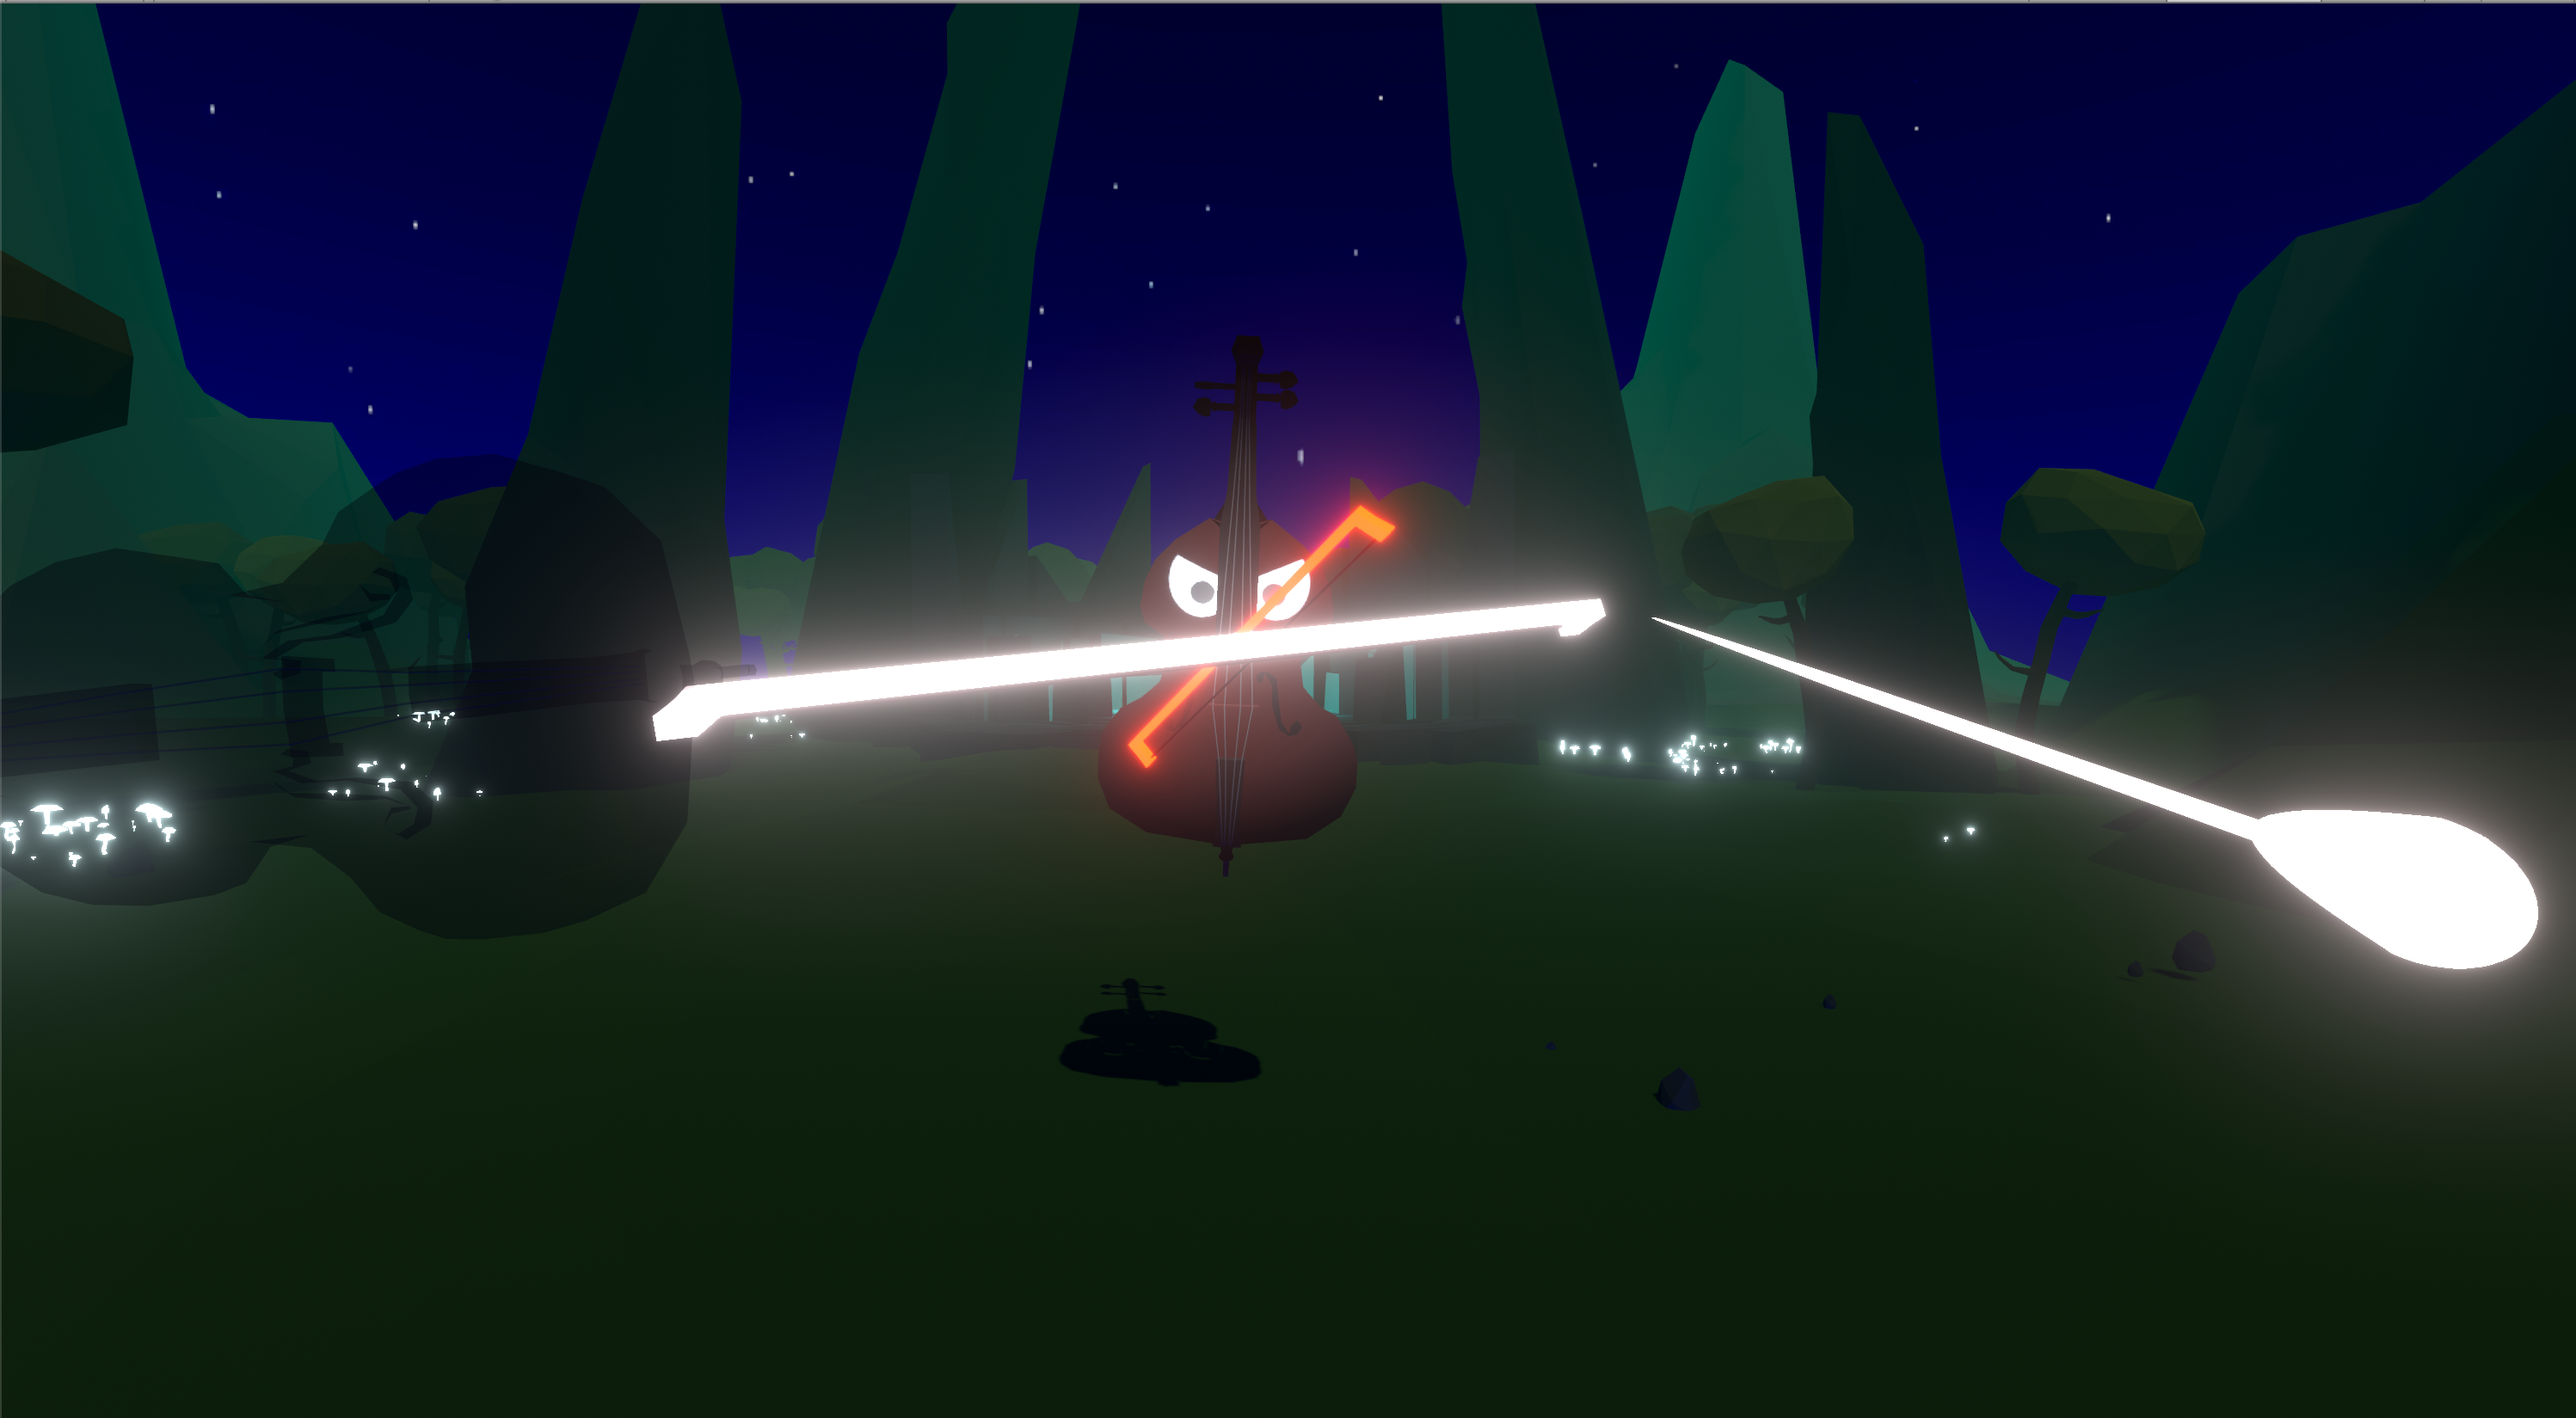
\includegraphics[width=0.75\textwidth]{figures/screenshots/contrabass.png}
    \caption[The Contrabass Distractor]{This screenshot shows off the contrabass distractor and its projectile attacks which travel directly towards the player.}
    \label{fig:contrabassDistractor}
\end{figure}
The first among the five distractor enemies is also the simplest one: ''The Contrabass'' as seen in Figure~\ref{fig:contrabassDistractor}. It attacks the player with projectiles that simply move towards them in a straight line. As a means to make the player move their head around more, the contrabass will mix slow and fast projectiles. A fast projectile will in this case move fast enough that it hits the player before a previously thrown slow projectile. This way, the player has to keep track of where the contrabass itself is when it uses fast projectiles while trying to remember where the slower moving ones are so they can absorb these as they come close. 
 
\subsection{The Oboe}
\begin{figure}[tbph]
    \centering
    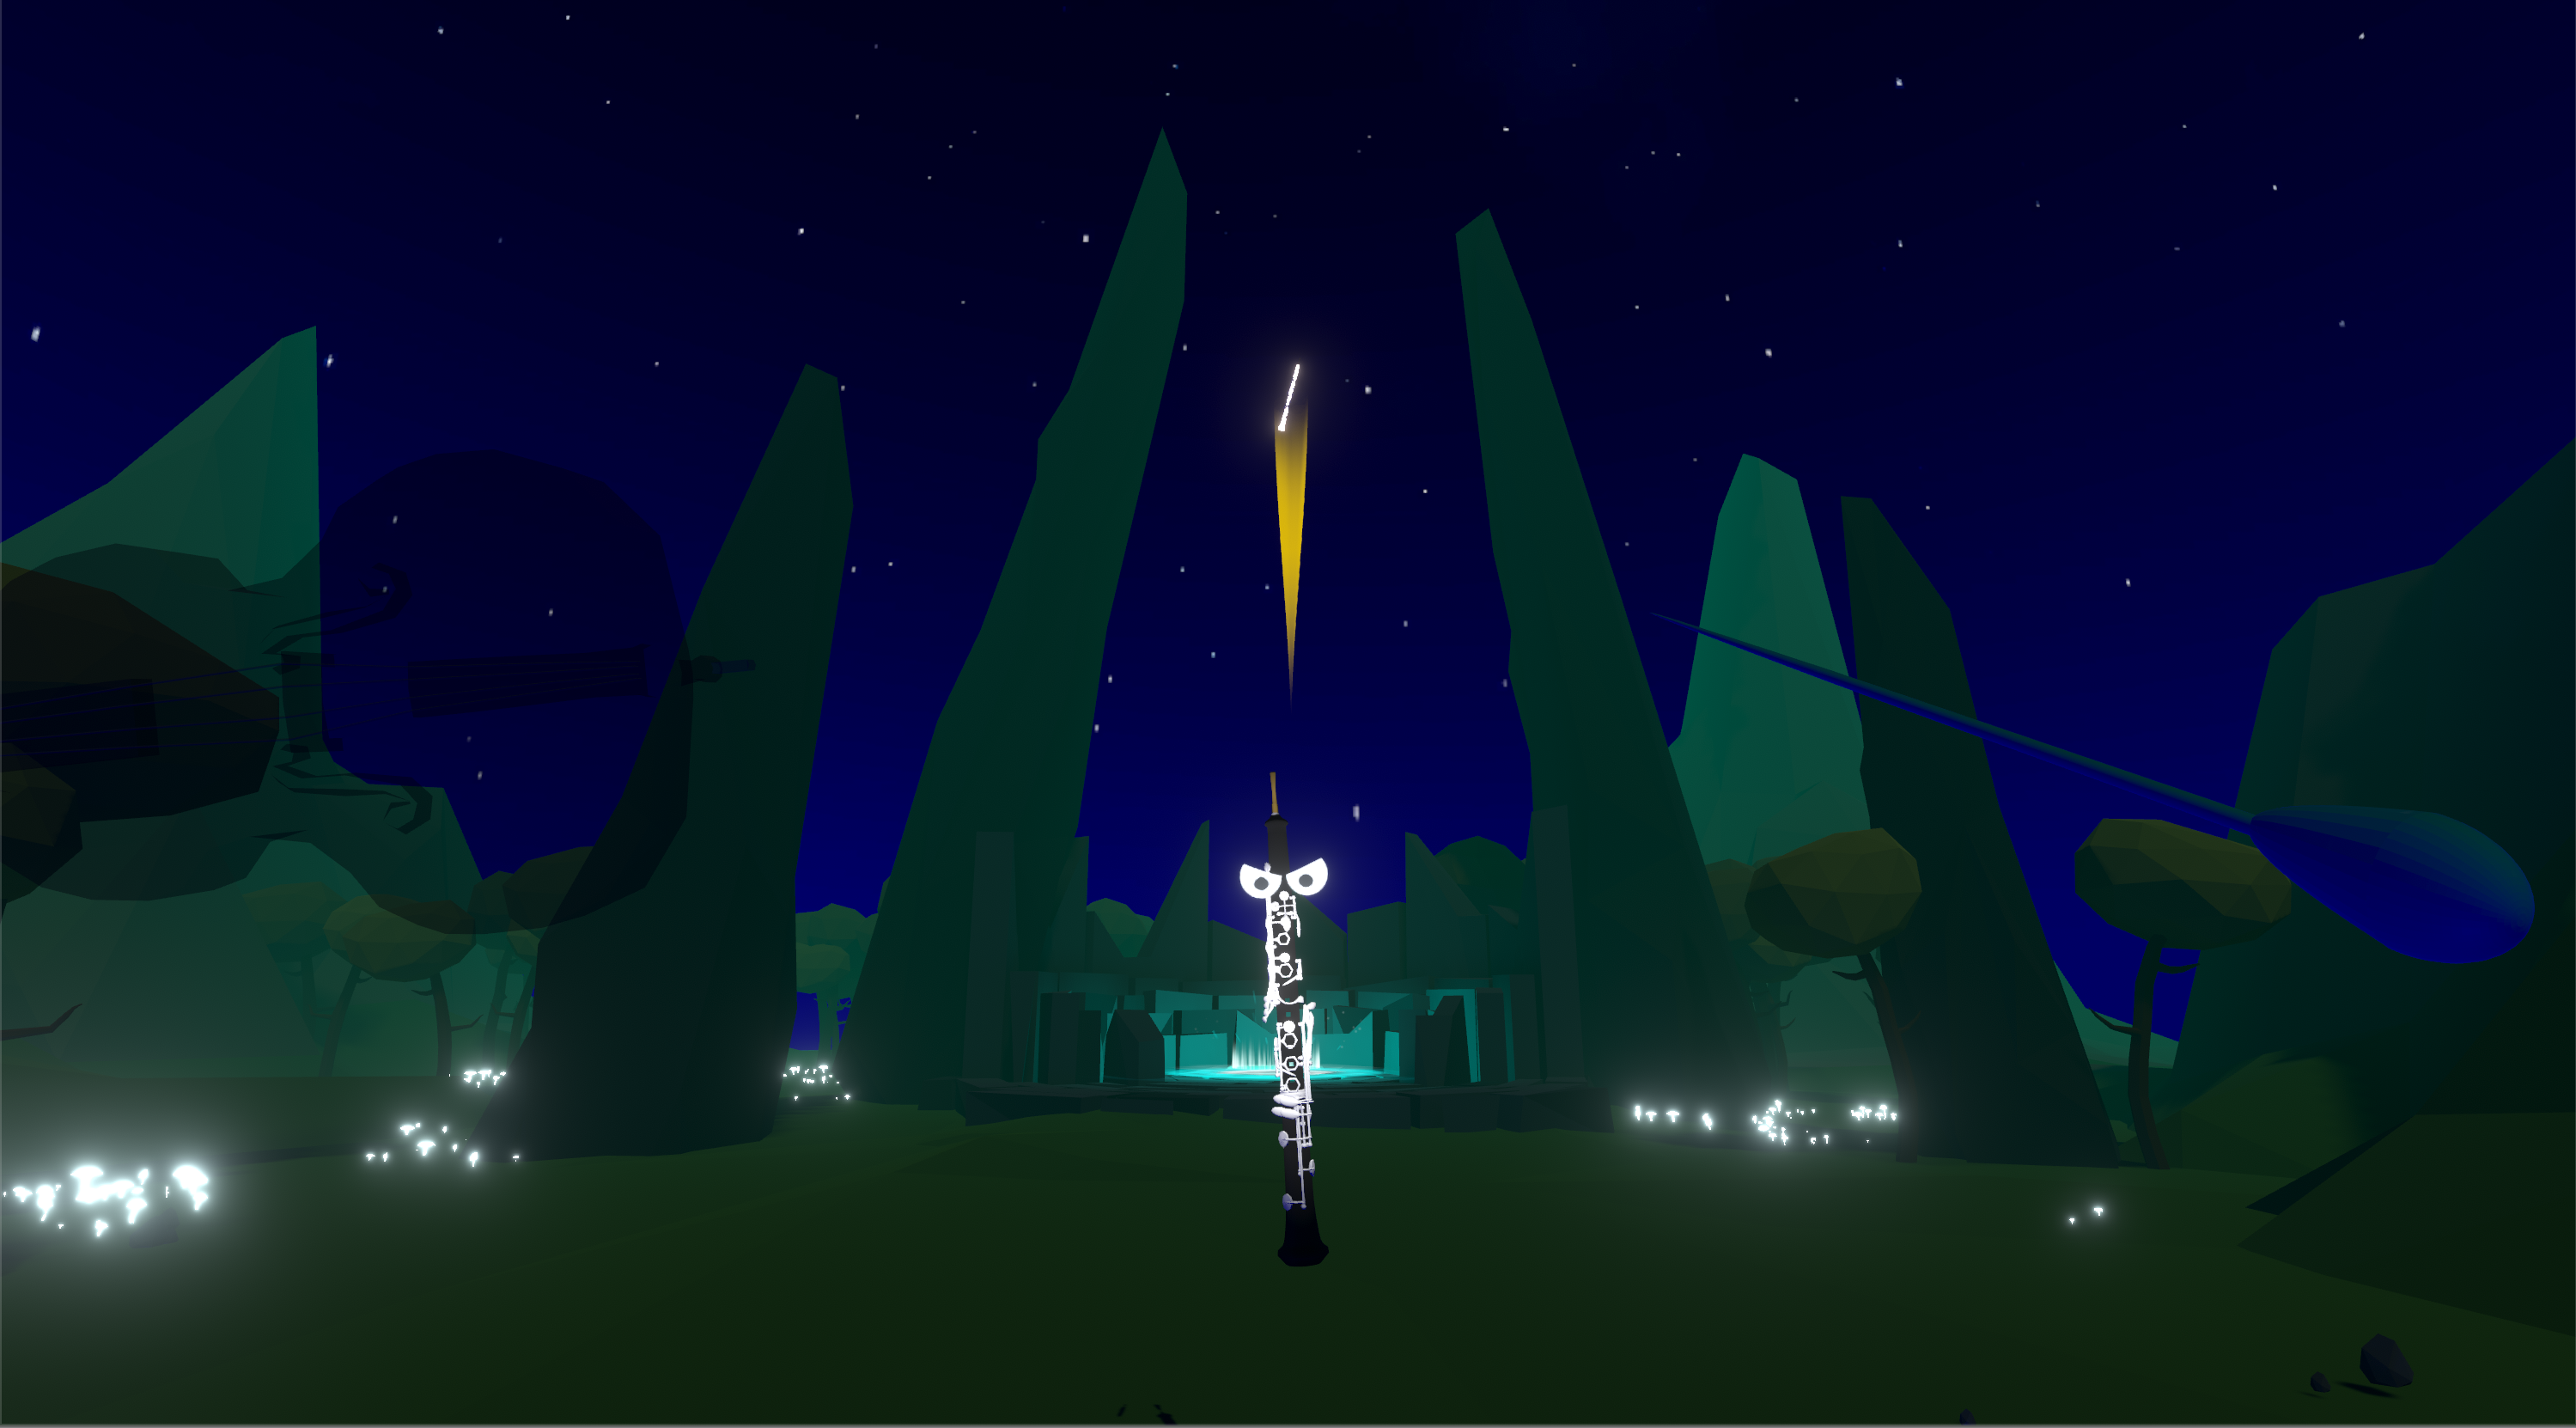
\includegraphics[width=0.75\textwidth]{figures/screenshots/oboe.png}
    \caption[The Oboe Distractor]{This screenshot shows the oboe distractor and its projectile attack which will travel on a vertical arc above the head of the player.}
    \label{fig:oboeDistractor}
\end{figure}

\begin{figure}[htbp]
  \centering
  \includesvg[width=0.5\textwidth]{figures/svgs/oboeProjectile.svg}
  \caption[Sideways 2D Example of Oboe Projectile Path]{An illustrated, sideways 2D example of how the oboe projectile travels. The blue circle and quad represents the player while the red circle represents the distractor that is about to attack.}
  \label{fig:oboeProjectile}
\end{figure}
The next distractor is ''The Oboe'' which can be seen in Figure~\ref{fig:oboeDistractor}. It attacks the player with projectiles that move in a vertical, 180 degree arc above the player's head before travelling straight towards their head. A rough two dimensional figure illustrating this can be found in Figure~\ref{fig:oboeProjectile}. The Oboe attempts to facilitate head rotation by trying to hit the player from behind with projectiles. A clever player might end up holding the shield behind their head to absorb these, lessening the impact of the approach though. Despite this, it is still necessary to keep track of the projectiles as the Oboe moves and rotates around the player. 

\subsection{The Harpsichord}
\begin{figure}[tbph]
    \centering
    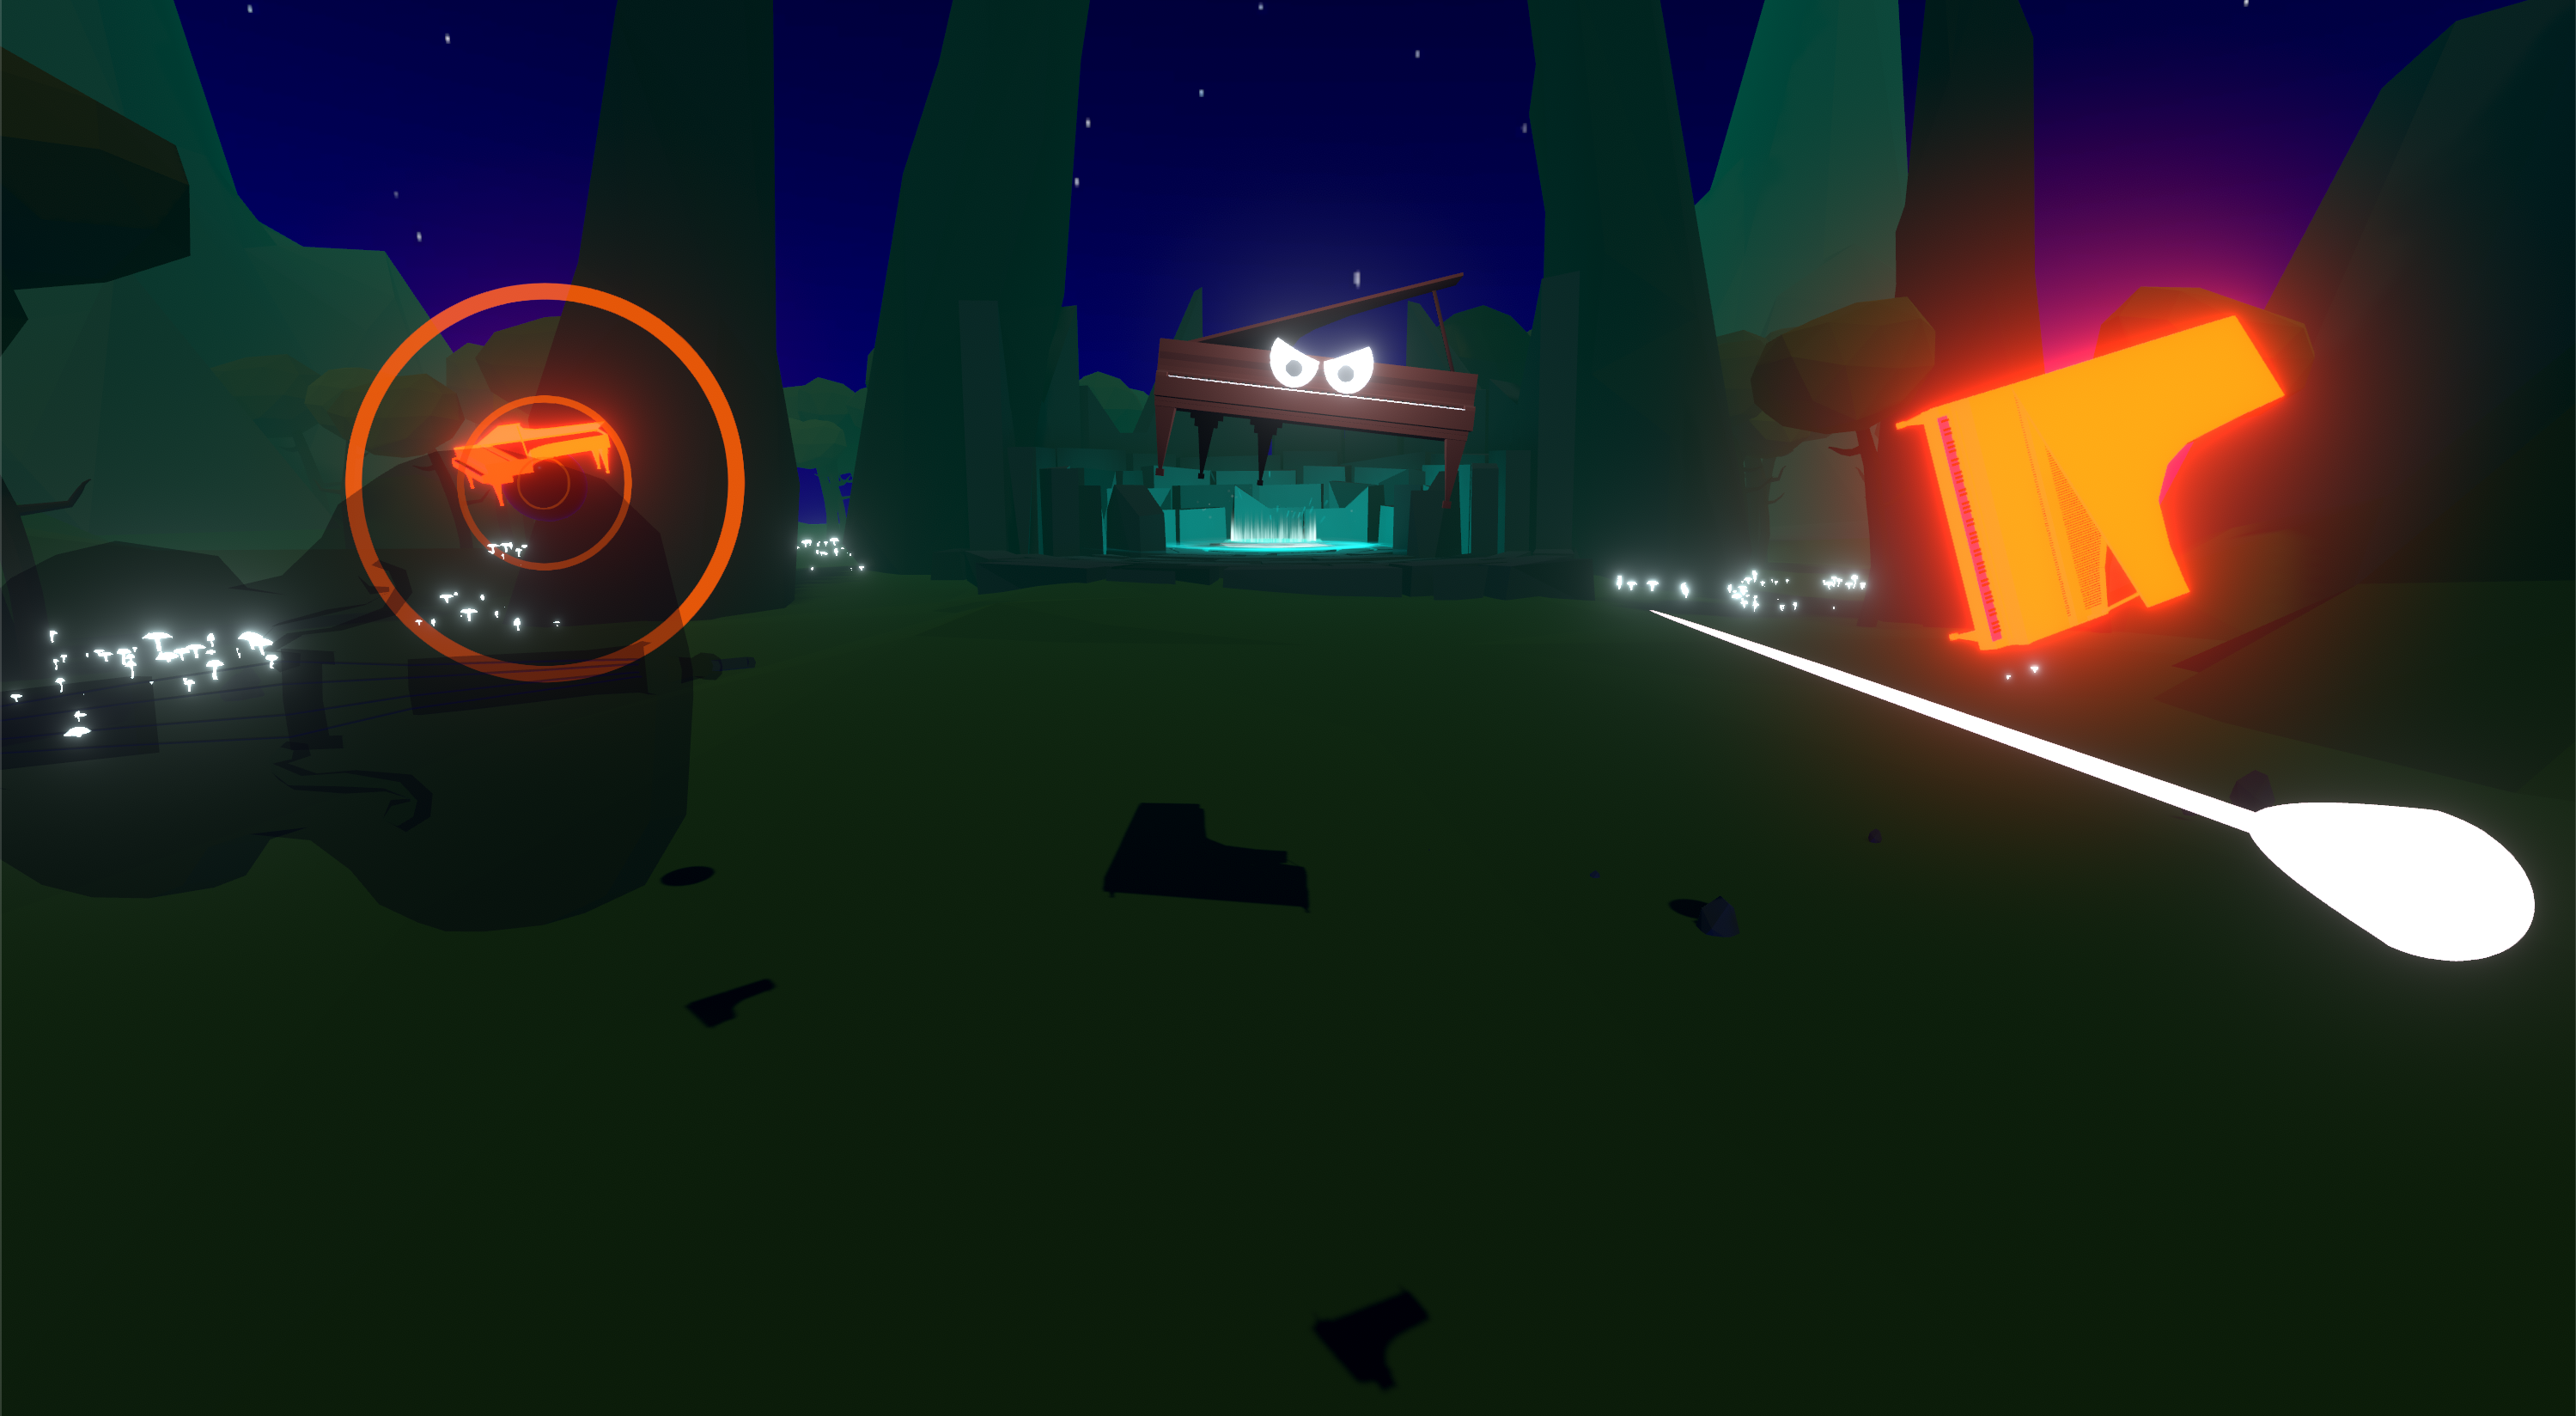
\includegraphics[width=0.75\textwidth]{figures/screenshots/harpsichord.png}
    \caption[The Harpsichord Distractor]{This screenshot shows the harpsichord distractor. It attacks with multiple rapid projectiles from two locations which are further away from its body.}
    \label{fig:harpsichordDistractor}
\end{figure}
''The Harpsichord'' which can be seen in Figure~\ref{fig:harpsichordDistractor} is the third distractor in Ensemble Retriever. It attacks the player with rapid projectiles that spawn from two wormholes that are further away from its body. This means that the player needs to move their shield from left to right to quickly block incoming projectiles. It allows for some extra head rotation as the player might need to slightly shift their head to clearly see each projectile. 

\subsection{The Violin}
\begin{figure}[tbph]
    \centering
    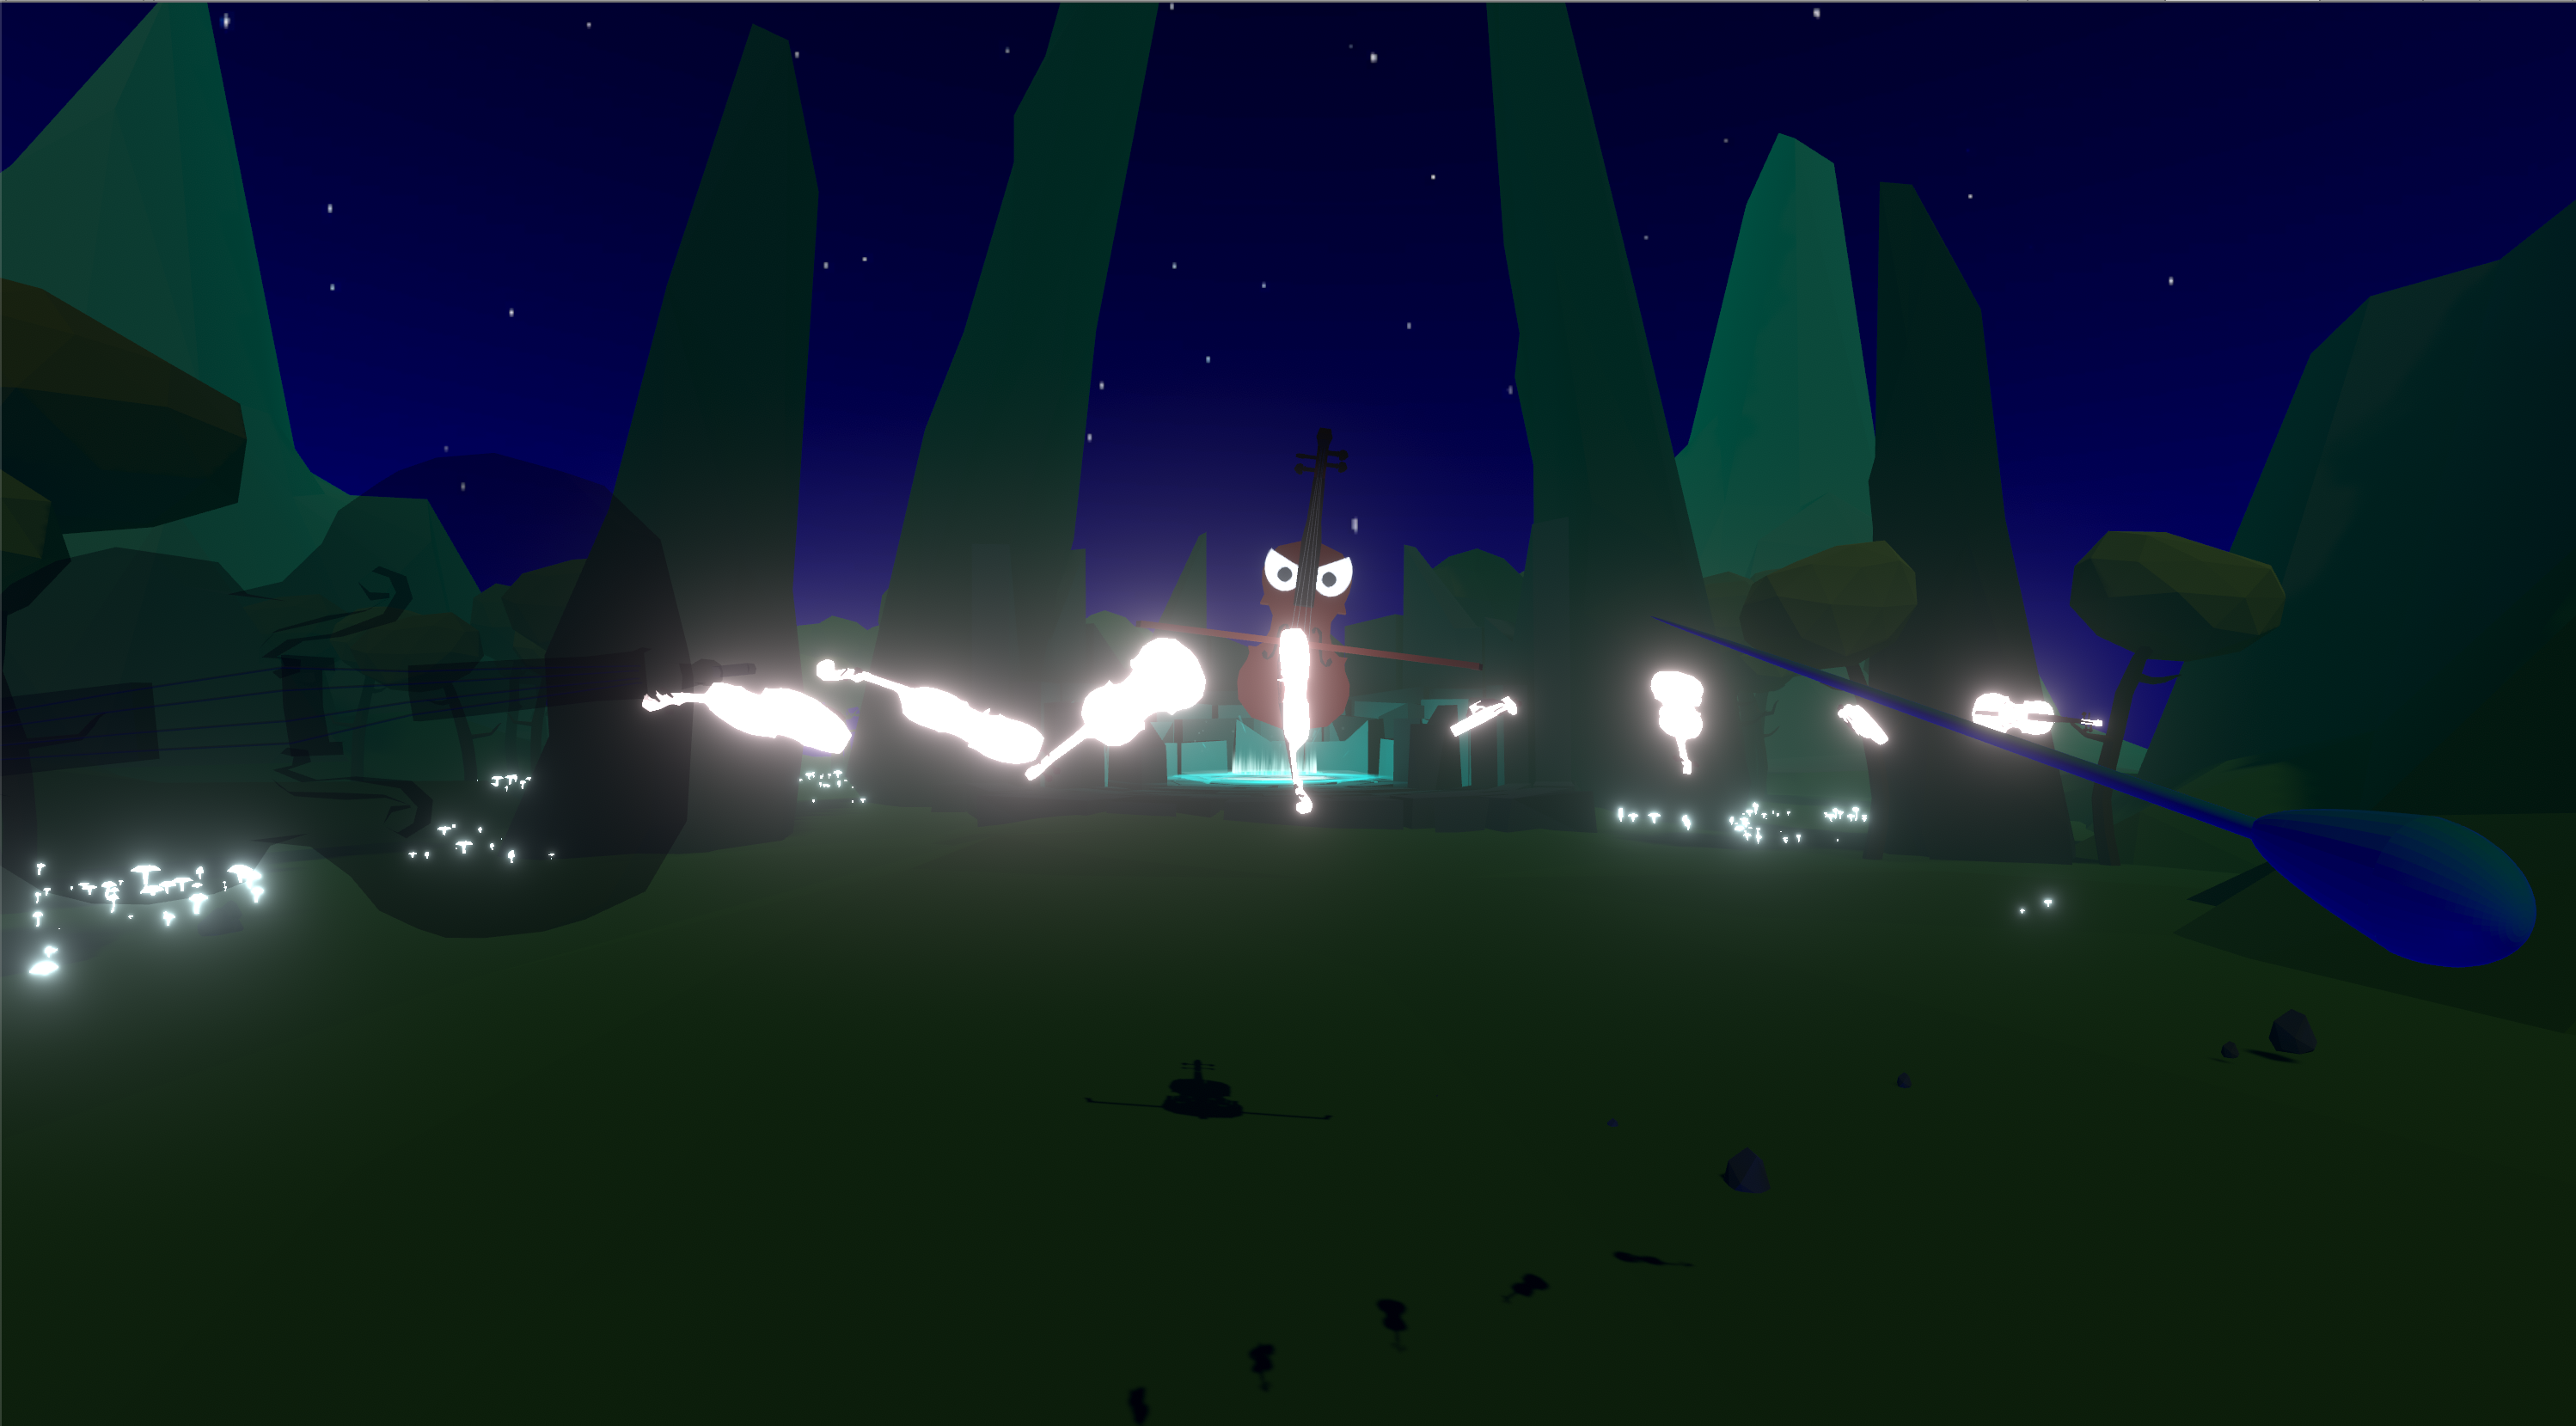
\includegraphics[width=0.75\textwidth]{figures/screenshots/violin.png}
    \caption[The Violin Distractor]{This screenshot shows the violin distractor. It attacks with several projectiles at a time in a line formation.}
    \label{fig:violinDistractor}
\end{figure}
The fourth distractor in Ensemble Retriever is ''The Violin'' which can be seen in Figure~\ref{fig:violinDistractor}. It is similar to the Harpsichord in the regard that it rapidly fires projectiles. Instead of firing projectiles from two locations though, it instead fires a line of projectiles that the player needs to block with their shield. This allows for some additional head rotation as the player needs to trace the line of projectiles that moves towards them. The line itself is long enough that some shifting of head orientation is beneficial to see everything as it gets close. 

\subsection{The Glockenspiel}
\begin{figure}[tbph]
    \centering
    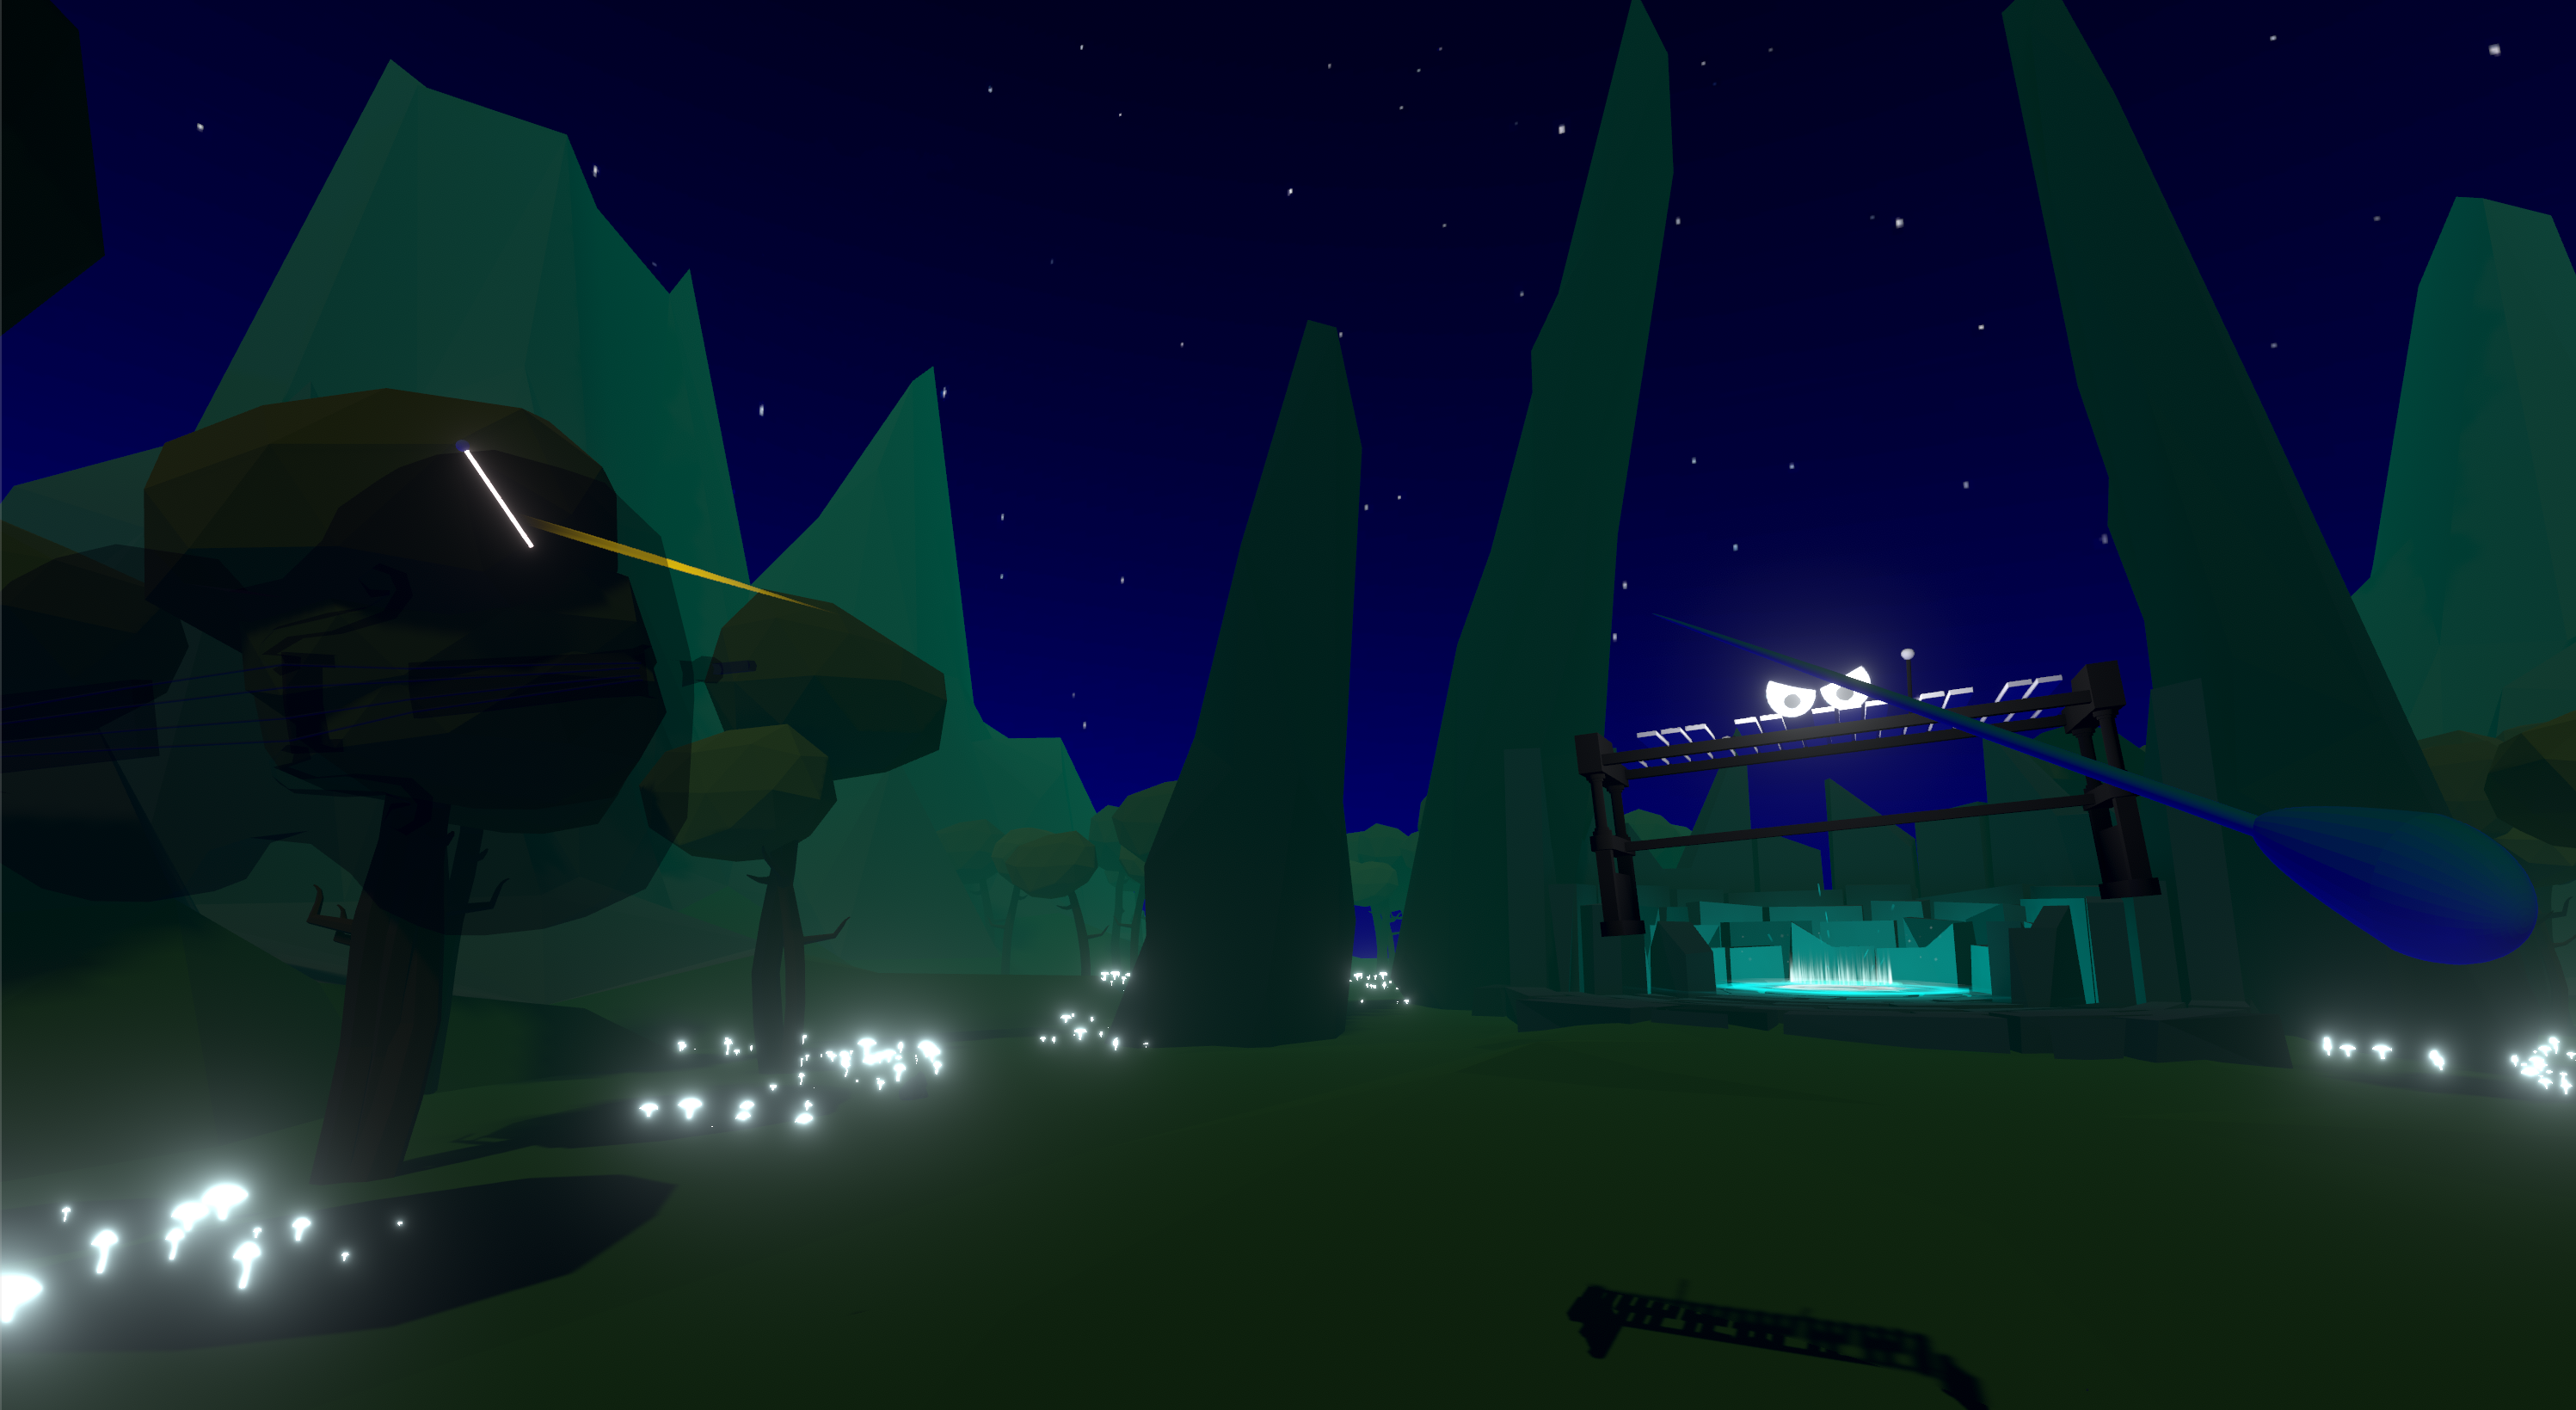
\includegraphics[width=0.75\textwidth]{figures/screenshots/glockenspiel.png}
    \caption[The Glockenspiel Distractor]{This screenshot shows the glockenspiel distractor and its curved projectile attack. The projectile itself travels on a \textasciitilde90 degree arc towards the player's left side.}
    \label{fig:glockenspielDistractor}
\end{figure}
Finally, we have ''The Glockenspiel'' which is seen in Figure~\ref{fig:glockenspielDistractor}. This distractor attacks the player by throwing projectiles that travel on a curve towards the player. The curve itself will intersect with the player at a roughly 90 degree angle to their left from where the projectile was fired. This facilitates more head rotation as the player needs to track the path that the projectile flies through before blocking. 

\section{Employing Context Sensitive Resets: Teleporters}
* Other researchers have looked into context sensitive reorientation outside of distractors haven't they? Double check!
* Can draw some comparisons to Suma et al.'s change blindness redirection.
   * Instead, in this case: it is possible to exploit the user's lack of knowledge with a future location to allow for reorientation. 
* As the player enters the portal, their facing direction after being teleported is changed in a manner so that the path they have to walk to continue is back towards the room centre.
* This is an example of an alternative context sensitive means of reorienting the user
* While it cannot be expected that a game is sprinkled with teleporters everywhere, this can be seen as a useful tool to use once in a while if you want to move the player to different locations and environments
* There are of course many other ways to also implement context sensitive resets. 
   * An elevator could for example be used for it
   * Anything in general that limits visibility or vision of the target destination can technically be used to create context sensitive reorientation in the same vein as this.
      * Very similar to what Sra et al. have already discussed in terms of limiting visibility for redirection and reorientation

\section{Disabling Redirected Walking Towards The End of an Experience}
* Throughout the final stretch of the game, redirection gains are disabled as a means of helping participants get used to normal head rotations before taking off the HMD.
* How effective this approach is, would of course need to be further tested in a separate study, but it should at least help somewhat normalise the head rotations for the user before finishing.
* Might not be easy to integrate with every solution, but in the case of Ensemble Retriever since the final portion is just to fight the Mountain King, there wont be much more movement involved so it is fine. 